\documentclass[a4paper]{book}
\usepackage{a4wide}
\usepackage{makeidx}
\usepackage{graphicx}
\usepackage{multicol}
\usepackage{float}
\usepackage{listings}
\usepackage{color}
\usepackage{textcomp}
\usepackage{alltt}
\usepackage{times}
\usepackage{ifpdf}
\ifpdf
\usepackage[pdftex,
            pagebackref=true,
            colorlinks=true,
            linkcolor=blue,
            unicode
           ]{hyperref}
\else
\usepackage[ps2pdf,
            pagebackref=true,
            colorlinks=true,
            linkcolor=blue,
            unicode
           ]{hyperref}
\usepackage{pspicture}
\fi
\usepackage[utf8]{inputenc}
\usepackage{doxygen}
\lstset{language=C++,inputencoding=utf8,basicstyle=\footnotesize,breaklines=true,breakatwhitespace=true,tabsize=4,numbers=left }
\makeindex
\setcounter{tocdepth}{3}
\renewcommand{\footrulewidth}{0.4pt}
\begin{document}
\hypersetup{pageanchor=false}
\begin{titlepage}
\vspace*{7cm}
\begin{center}
{\Large Intel Hex Encoder/Decoder Class }\\
\vspace*{1cm}
{\large Generated by Doxygen 1.7.1}\\
\vspace*{0.5cm}
{\small Mon Jan 9 2012 09:36:42}\\
\end{center}
\end{titlepage}
\clearemptydoublepage
\pagenumbering{roman}
\tableofcontents
\clearemptydoublepage
\pagenumbering{arabic}
\hypersetup{pageanchor=true}
\chapter{Class Index}
\section{Class List}
Here are the classes, structs, unions and interfaces with brief descriptions:\begin{DoxyCompactList}
\item\contentsline{section}{\hyperlink{classintelhex}{intelhex} (Class to decode, encode and manipulate Intel HEX format files )}{\pageref{classintelhex}}{}
\end{DoxyCompactList}

\chapter{File Index}
\section{File List}
Here is a list of all documented files with brief descriptions:\begin{DoxyCompactList}
\item\contentsline{section}{{\bfseries intelhexclass.cpp} }{\pageref{intelhexclass_8cpp}}{}
\item\contentsline{section}{\hyperlink{intelhexclass_8hpp}{intelhexclass.hpp} }{\pageref{intelhexclass_8hpp}}{}
\end{DoxyCompactList}

\chapter{Class Documentation}
\hypertarget{classintelhex}{
\section{intelhex Class Reference}
\label{classintelhex}\index{intelhex@{intelhex}}
}


Class to decode, encode and manipulate Intel HEX format files.  




{\ttfamily \#include $<$intelhexclass.hpp$>$}



Collaboration diagram for intelhex:
\nopagebreak
\begin{figure}[H]
\begin{center}
\leavevmode
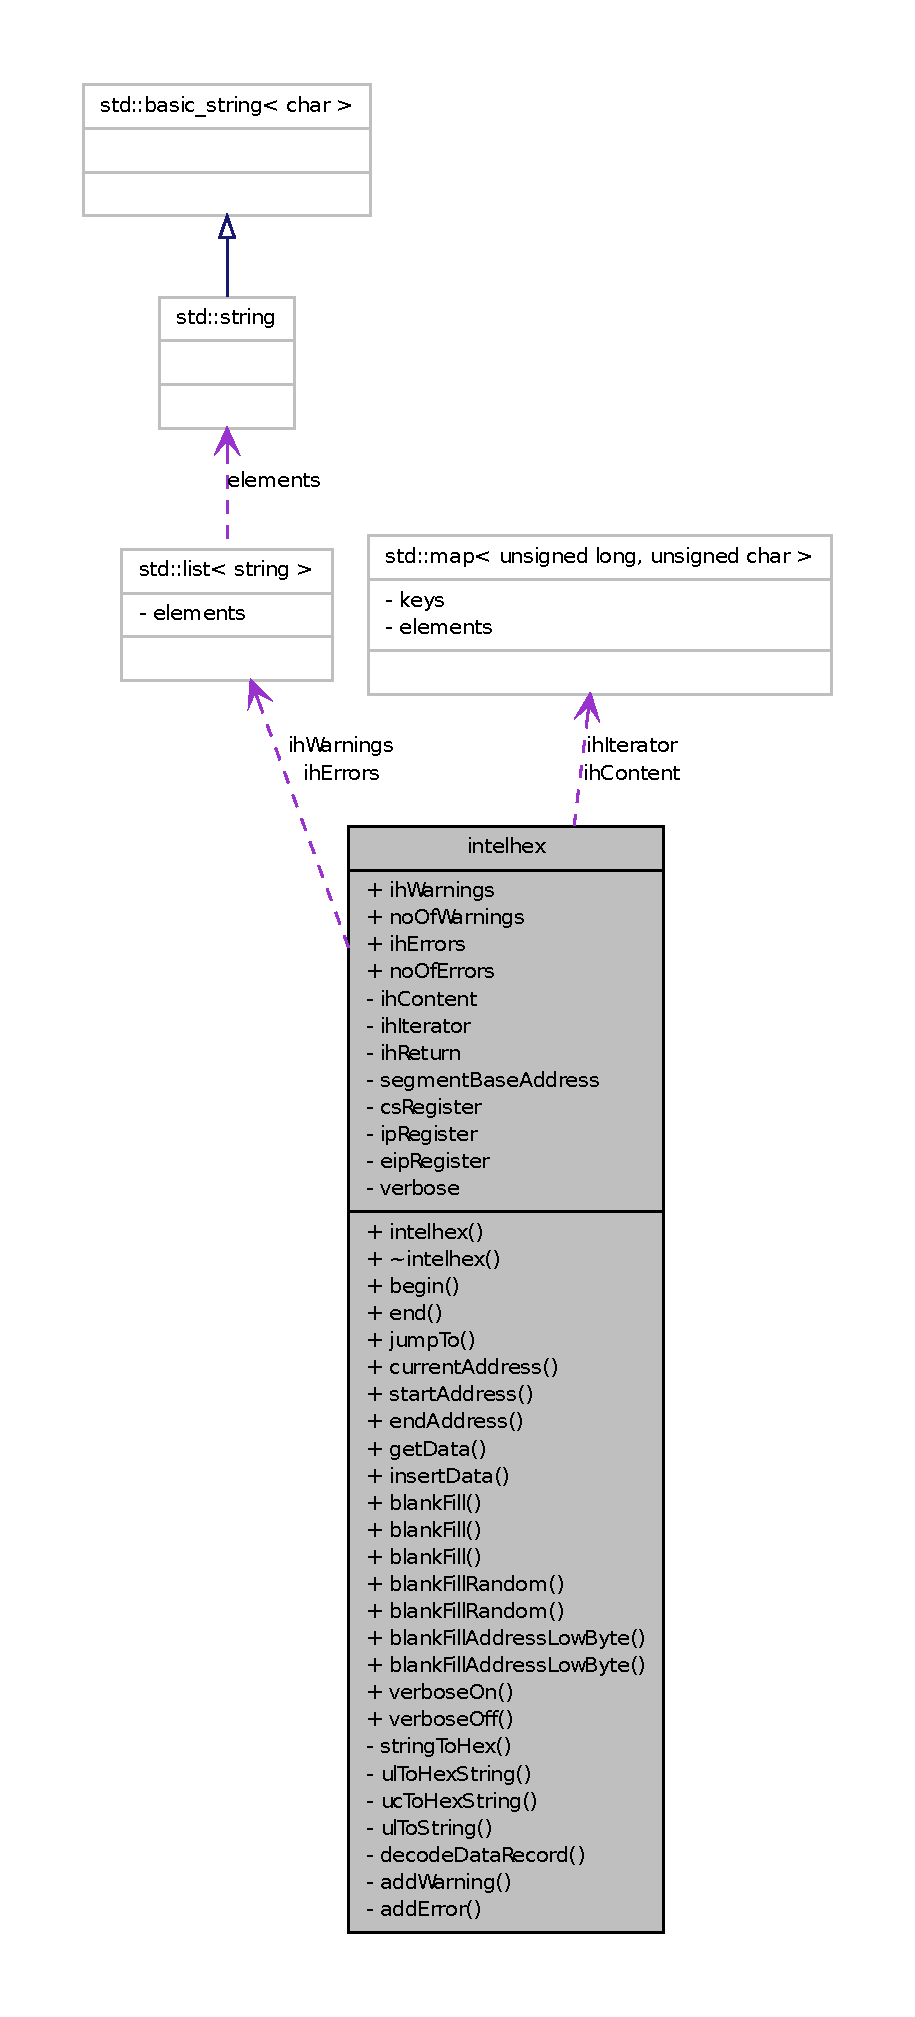
\includegraphics[width=400pt]{classintelhex__coll__graph}
\end{center}
\end{figure}
\subsection*{Public Member Functions}
\begin{DoxyCompactItemize}
\item 
\hypertarget{classintelhex_ab2b1119e14a960ea2b356967244aafb3}{
void {\bfseries begin} ()}
\label{classintelhex_ab2b1119e14a960ea2b356967244aafb3}

\item 
\hypertarget{classintelhex_a7759926596cfcffec94e391fff4298e9}{
void {\bfseries end} ()}
\label{classintelhex_a7759926596cfcffec94e391fff4298e9}

\item 
\hypertarget{classintelhex_a83b54457c121b0f35b21b78fa2ecd712}{
bool {\bfseries jumpTo} (unsigned long address)}
\label{classintelhex_a83b54457c121b0f35b21b78fa2ecd712}

\item 
\hypertarget{classintelhex_a631d8930daeaf04bf0d9ad9c25679a0b}{
unsigned long {\bfseries currentAddress} ()}
\label{classintelhex_a631d8930daeaf04bf0d9ad9c25679a0b}

\item 
\hypertarget{classintelhex_ab78b6ecc1fd3889bfb0c3bb57f028a64}{
unsigned long {\bfseries startAddress} ()}
\label{classintelhex_ab78b6ecc1fd3889bfb0c3bb57f028a64}

\item 
\hypertarget{classintelhex_af7692acb24330da3debf8c7fb21ab056}{
unsigned long {\bfseries endAddress} ()}
\label{classintelhex_af7692acb24330da3debf8c7fb21ab056}

\item 
\hypertarget{classintelhex_a00e0fd557bec34d0bb11ef92530121a0}{
unsigned char {\bfseries getData} ()}
\label{classintelhex_a00e0fd557bec34d0bb11ef92530121a0}

\item 
\hypertarget{classintelhex_a71096983db3c24a5ac9b95663937a4ce}{
bool {\bfseries insertData} (unsigned char data)}
\label{classintelhex_a71096983db3c24a5ac9b95663937a4ce}

\item 
\hypertarget{classintelhex_a5de5cf10103fc307127f9017f3e5cd76}{
bool {\bfseries blankFill} (unsigned char data)}
\label{classintelhex_a5de5cf10103fc307127f9017f3e5cd76}

\item 
\hypertarget{classintelhex_a84bbd449bb55e218b62ea73e2b399196}{
bool {\bfseries blankFill} (unsigned char $\ast$const data, unsigned long sizeOfData)}
\label{classintelhex_a84bbd449bb55e218b62ea73e2b399196}

\item 
\hypertarget{classintelhex_aaf6f77af7a82623ef16471f105ac3fe7}{
void {\bfseries blankFill} (unsigned char $\ast$const data, unsigned long sizeOfData, unsigned long endAddress)}
\label{classintelhex_aaf6f77af7a82623ef16471f105ac3fe7}

\item 
\hypertarget{classintelhex_a9c26ba3dc9dd4f3021bb6c7f6983388f}{
bool {\bfseries blankFillRandom} ()}
\label{classintelhex_a9c26ba3dc9dd4f3021bb6c7f6983388f}

\item 
\hypertarget{classintelhex_aa1dbcbf3df1aaafd518882c882f43f76}{
void {\bfseries blankFillRandom} (unsigned long endAddress)}
\label{classintelhex_aa1dbcbf3df1aaafd518882c882f43f76}

\item 
\hypertarget{classintelhex_a2e5c67fccc34c78e6dbd28f4b795fb0f}{
bool {\bfseries blankFillAddressLowByte} ()}
\label{classintelhex_a2e5c67fccc34c78e6dbd28f4b795fb0f}

\item 
\hypertarget{classintelhex_ab7b16f457563da93569b9812fafb9e7d}{
void {\bfseries blankFillAddressLowByte} (unsigned long endAddress)}
\label{classintelhex_ab7b16f457563da93569b9812fafb9e7d}

\item 
\hypertarget{classintelhex_ac6a0119a04a2090af3ffe8c33a37cbc9}{
void {\bfseries verboseOn} ()}
\label{classintelhex_ac6a0119a04a2090af3ffe8c33a37cbc9}

\item 
\hypertarget{classintelhex_a3958f077a662291bbde3472ea2bcfb4d}{
void {\bfseries verboseOff} ()}
\label{classintelhex_a3958f077a662291bbde3472ea2bcfb4d}

\end{DoxyCompactItemize}
\subsection*{Public Attributes}
\begin{DoxyCompactItemize}
\item 
\hypertarget{classintelhex_a0ae0e9a75bdfaa50d6d0266bb3d56ed1}{
list$<$ string $>$ {\bfseries ihWarnings}}
\label{classintelhex_a0ae0e9a75bdfaa50d6d0266bb3d56ed1}

\item 
\hypertarget{classintelhex_a5ea3789cc9ea71c9b35322aabca05158}{
unsigned long {\bfseries noOfWarnings}}
\label{classintelhex_a5ea3789cc9ea71c9b35322aabca05158}

\item 
\hypertarget{classintelhex_a76fb4550b43dfbb08018cabf34298400}{
list$<$ string $>$ {\bfseries ihErrors}}
\label{classintelhex_a76fb4550b43dfbb08018cabf34298400}

\item 
\hypertarget{classintelhex_a451b78972165b898e91a129670fce919}{
unsigned long {\bfseries noOfErrors}}
\label{classintelhex_a451b78972165b898e91a129670fce919}

\end{DoxyCompactItemize}
\subsection*{Friends}
\begin{DoxyCompactItemize}
\item 
ostream \& \hyperlink{classintelhex_aad8e829c665b49d225a9d0dc48c1fe3c}{operator$<$$<$} (ostream \&dataOut, const \hyperlink{classintelhex}{intelhex} \&ihLocal)
\item 
istream \& \hyperlink{classintelhex_a73fb9c5b9d6d069b5eb83340942fd54b}{operator$>$$>$} (istream \&dataIn, \hyperlink{classintelhex}{intelhex} \&ihLocal)
\end{DoxyCompactItemize}


\subsection{Detailed Description}
Class to decode, encode and manipulate Intel HEX format files. The Intel HEX class allows the user to stream in the content of an Intel HEX file so that its content can by analysed more easily than trying to decode the Intel HEX file in a text editor. In conjunction with a suitable application it is possible to create content, analyse content and even compare the content of files with one another. 

Definition at line 83 of file intelhexclass.hpp.



\subsection{Friends And Related Function Documentation}
\hypertarget{classintelhex_aad8e829c665b49d225a9d0dc48c1fe3c}{
\index{intelhex@{intelhex}!operator$<$$<$@{operator$<$$<$}}
\index{operator$<$$<$@{operator$<$$<$}!intelhex@{intelhex}}
\subsubsection[{operator$<$$<$}]{\setlength{\rightskip}{0pt plus 5cm}ostream\& operator$<$$<$ (
\begin{DoxyParamCaption}
\item[{ostream \&}]{ dataOut, }
\item[{const {\bf intelhex} \&}]{ ihLocal}
\end{DoxyParamCaption}
)\hspace{0.3cm}{\ttfamily  \mbox{[}friend\mbox{]}}}}
\label{classintelhex_aad8e829c665b49d225a9d0dc48c1fe3c}
Output stream overload operator Operator overloaded to encode any data held in memory into the Intel HEX format for storage on disk

\begin{DoxySeeAlso}{See also}
\hyperlink{classintelhex_a73fb9c5b9d6d069b5eb83340942fd54b}{operator$>$$>$()}
\end{DoxySeeAlso}

\begin{DoxyParams}{Parameters}
\item[{\em dataOut}]-\/ Output stream for to store the decoded file information \item[{\em ihLocal}]-\/ Points to this class so that friend function has access to private class members \end{DoxyParams}
\hypertarget{classintelhex_a73fb9c5b9d6d069b5eb83340942fd54b}{
\index{intelhex@{intelhex}!operator$>$$>$@{operator$>$$>$}}
\index{operator$>$$>$@{operator$>$$>$}!intelhex@{intelhex}}
\subsubsection[{operator$>$$>$}]{\setlength{\rightskip}{0pt plus 5cm}istream\& operator$>$$>$ (
\begin{DoxyParamCaption}
\item[{istream \&}]{ dataIn, }
\item[{{\bf intelhex} \&}]{ ihLocal}
\end{DoxyParamCaption}
)\hspace{0.3cm}{\ttfamily  \mbox{[}friend\mbox{]}}}}
\label{classintelhex_a73fb9c5b9d6d069b5eb83340942fd54b}
Input stream overload operator Operator overloaded to decode data streamed in from a file in the Intel HEX format into memory

\begin{DoxySeeAlso}{See also}
\hyperlink{classintelhex_aad8e829c665b49d225a9d0dc48c1fe3c}{operator$<$$<$()}
\end{DoxySeeAlso}

\begin{DoxyParams}{Parameters}
\item[{\em dataIn}]-\/ Input stream for the encoded file information \item[{\em ihLocal}]-\/ Points to this class so that friend function has access to private class members \end{DoxyParams}


Definition at line 211 of file intelhexclass.cpp.




\begin{DoxyCode}
{
    // Create a string to store lines of Intel Hex info
    string ihLine;
    /* Create a string to store a single byte of Intel HEX info               */
    string ihByte;
    // Create an iterator for this variable
    string::iterator ihLineIterator;
    // Create a line counter
    unsigned long lineCounter = 0;
    // Variable to hold a single byte (two chars) of data
    unsigned char byteRead;
    // Variable to calculate the checksum for each line
    unsigned char intelHexChecksum;
    // Variable to hold the record length
    unsigned char recordLength;
    // Variable to hold the load offset
    unsigned long loadOffset;
    // Variables to hold the record type
    intelhexRecordType recordType;
    
    do
    {
        /* Clear the string before this next round                            */
        ihLine.erase();
        
        /* Clear the checksum before processing this line                     */
        intelHexChecksum = 0;
        
        /* Get a line of data                                                 */
        dataIn >> ihLine;
        
        /* If the line contained some data, process it                        */
        if (ihLine.length() > 0)
        {
            /* Increment line counter                                         */
            lineCounter++;
        
            /* Set string iterator to start of string                         */
            ihLineIterator = ihLine.begin();
        
            /* Check that we have a ':' record mark at the beginning          */
            if (*ihLineIterator != ':')
            {
                /* Add some warning code here                                 */
                string message;

                message = "Line without record mark ':' found @ line " +
                                                ihLocal.ulToString(lineCounter);

                ihLocal.addWarning(message);
            }
        
            /* Remove the record mark from the string as we don't need it     */
            /* anymore                                                        */
            ihLine.erase(ihLineIterator);
        
            /* Run through the whole line to check the checksum               */
            for (ihLineIterator = ihLine.begin(); 
                 ihLineIterator != ihLine.end(); 
                 /* Nothing - really! */ )
            {
                /* Convert the line in pair of chars (making a single byte)   */
                /* into single bytes, and then add to the checksum variable.  */
                /* By adding all the bytes in a line together *including* the */
                /* checksum byte, we should get a result of '0' at the end.   */
                /* If not, there is a checksum error                          */
                ihByte.erase();
                
                ihByte = *ihLineIterator;
                ++ihLineIterator;
                /* Just in case there are an odd number of chars in the       */
                /* just check we didn't reach the end of the string early     */
                if (ihLineIterator != ihLine.end())
                {
                    ihByte += *ihLineIterator;
                    ++ihLineIterator;
                
                    byteRead = ihLocal.stringToHex(ihByte);
                           
                    intelHexChecksum += byteRead;
                }
                else
                {
                    string message;
                            
                    message = "Odd number of characters in line " +
                                                ihLocal.ulToString(lineCounter);
                            
                    ihLocal.addError(message);
                }
            }
        
            /* Make sure the checksum was ok                                  */
            if (intelHexChecksum == 0)
            {
                /* Reset iterator back to beginning of the line so we can now */
                /* decode it                                                  */
                ihLineIterator = ihLine.begin();
                
                /* Clear all the variables associated with decoding a line of */
                /* Intel HEX code.                                            */
                recordLength = 0;
                loadOffset = 0;
                
                /* Get the record length                                      */
                ihByte.erase();
                ihByte = *ihLineIterator;
                ++ihLineIterator;
                ihByte += *ihLineIterator;
                ++ihLineIterator;
                recordLength = ihLocal.stringToHex(ihByte);
                
                /* Get the load offset (2 bytes)                              */
                ihByte.erase();
                ihByte = *ihLineIterator;
                ++ihLineIterator;
                ihByte += *ihLineIterator;
                ++ihLineIterator;
                loadOffset = 
                        static_cast<unsigned long>(ihLocal.stringToHex(ihByte));
                loadOffset <<= 8;
                ihByte.erase();
                ihByte = *ihLineIterator;
                ++ihLineIterator;
                ihByte += *ihLineIterator;
                ++ihLineIterator;
                loadOffset += 
                        static_cast<unsigned long>(ihLocal.stringToHex(ihByte));
                
                /* Get the record type                                        */
                ihByte.erase();
                ihByte = *ihLineIterator;
                ++ihLineIterator;
                ihByte += *ihLineIterator;
                ++ihLineIterator;
                recordType = 
                   static_cast<intelhexRecordType>(ihLocal.stringToHex(ihByte));
                           
                /* Decode the INFO or DATA portion of the record              */
                switch (recordType)
                {
                    case DATA_RECORD:
                        ihLocal.decodeDataRecord(recordLength, loadOffset,
                                                 ihLineIterator);
                        if (ihLocal.verbose == true)
                        {
                            cout << "Data Record begining @ 0x" << 
                                      ihLocal.ulToHexString(loadOffset) << endl;
                        }
                        break;
                    
                    case END_OF_FILE_RECORD:
                        /* Note the line number at this point. Later, check   */
                        /* that there were no more lines after this one.      */
                        /* Generate error if there were                       */
                        if (ihLocal.verbose == true)
                        {
                            cout << "End of File" << endl;
                        }
                        break;
                        
                    case EXTENDED_SEGMENT_ADDRESS:
                        /* Make sure we have 2 bytes of data                  */
                        if (recordLength == 2)
                        {
                            /* Extract the two bytes of the ESA               */
                            unsigned long extSegAddress = 0;
                            
                            ihByte.erase();
                            ihByte = *ihLineIterator;
                            ++ihLineIterator;
                            ihByte += *ihLineIterator;
                            ++ihLineIterator;
                            extSegAddress = static_cast<unsigned long>
                                                  (ihLocal.stringToHex(ihByte));
                            extSegAddress <<= 8;
                            ihByte.erase();
                            ihByte = *ihLineIterator;
                            ++ihLineIterator;
                            ihByte += *ihLineIterator;
                            ++ihLineIterator;
                            extSegAddress += static_cast<unsigned long>
                                                  (ihLocal.stringToHex(ihByte));
                            
                            /* ESA is bits 4-19 of the segment base address   */
                            /* (SBA), so shift left 4 bits                    */
                            extSegAddress <<= 4;
                            
                            /* Update the SBA                                 */
                            ihLocal.segmentBaseAddress = extSegAddress;
                        }
                        else
                        {
                            /* Note the error                                 */
                            string message;
                            
                            message = "Extended Segment Address @ line " +
                                      ihLocal.ulToString(lineCounter) + 
                                      " not 2 bytes as required.";
                            
                            ihLocal.addError(message);
                        }
                        if (ihLocal.verbose == true)
                        {
                            cout << "Ext. Seg. Address found: 0x" <<
                               ihLocal.ulToHexString(ihLocal.segmentBaseAddress)
                                                                        << endl;
                        }
                        
                        break;
                        
                    case START_SEGMENT_ADDRESS:
                        /* Make sure we have 4 bytes of data                  */
                        if (recordLength == 4)
                        {
                            ihLocal.csRegister = 0;
                            ihLocal.ipRegister = 0;
                            
                            ihByte.erase();
                            ihByte = *ihLineIterator;
                            ++ihLineIterator;
                            ihByte += *ihLineIterator;
                            ++ihLineIterator;
                            ihLocal.csRegister = static_cast<unsigned long>
                                                  (ihLocal.stringToHex(ihByte));
                            ihLocal.csRegister <<= 8;
                            ihByte.erase();
                            ihByte = *ihLineIterator;
                            ++ihLineIterator;
                            ihByte += *ihLineIterator;
                            ++ihLineIterator;
                            ihLocal.csRegister += static_cast<unsigned long>
                                                  (ihLocal.stringToHex(ihByte));
                                
                            ihByte.erase();
                            ihByte = *ihLineIterator;
                            ++ihLineIterator;
                            ihByte += *ihLineIterator;
                            ++ihLineIterator;
                            ihLocal.ipRegister = static_cast<unsigned long>
                                                  (ihLocal.stringToHex(ihByte));
                            ihLocal.ipRegister <<= 8;
                            ihByte.erase();
                            ihByte = *ihLineIterator;
                            ++ihLineIterator;
                            ihByte += *ihLineIterator;
                            ++ihLineIterator;
                            ihLocal.ipRegister += static_cast<unsigned long>
                                                  (ihLocal.stringToHex(ihByte));
                        }
                        else
                        {
                            /* Note the error                                 */
                            //cout << "Error in Start Seg. Address" << endl;
                            
                            string message;
                            
                            message = "Start Segment Address @ line " +
                                      ihLocal.ulToString(lineCounter) + 
                                      " not 4 bytes as required.";
                            
                            ihLocal.addError(message);
                        }
                        if (ihLocal.verbose == true)
                        {
                            cout << "Start Seg. Address - CS 0x" <<
                                 ihLocal.ulToHexString(ihLocal.csRegister) <<
                                 " IP 0x" << 
                                 ihLocal.ulToHexString(ihLocal.ipRegister) 
                                                                        << endl;
                        }
                        break;
                        
                    case EXTENDED_LINEAR_ADDRESS:
                        /* Make sure we have 2 bytes of data                  */
                        if (recordLength == 2)
                        {
                            /* Extract the two bytes of the ELA               */
                            unsigned long extLinAddress = 0;
                            
                            ihByte.erase();
                            ihByte = *ihLineIterator;
                            ++ihLineIterator;
                            ihByte += *ihLineIterator;
                            ++ihLineIterator;
                            extLinAddress = static_cast<unsigned long>
                                                  (ihLocal.stringToHex(ihByte));
                            extLinAddress <<= 8;
                            ihByte.erase();
                            ihByte = *ihLineIterator;
                            ++ihLineIterator;
                            ihByte += *ihLineIterator;
                            ++ihLineIterator;
                            extLinAddress += static_cast<unsigned long>
                                                  (ihLocal.stringToHex(ihByte));
                            
                            /* ELA is bits 16-31 of the segment base address  */
                            /* (SBA), so shift left 16 bits                   */
                            extLinAddress <<= 16;
                            
                            /* Update the SBA                                 */
                            ihLocal.segmentBaseAddress = extLinAddress;
                        }
                        else
                        {
                            /* Note the error                                 */
                            //cout << "Error in Ext. Lin. Address" << endl;
                            
                            string message;
                            
                            message = "Extended Linear Address @ line " +
                                      ihLocal.ulToString(lineCounter) + 
                                      " not 2 bytes as required.";
                            
                            ihLocal.addError(message);
                        }
                        if (ihLocal.verbose == true)
                        {
                            cout << "Ext. Lin. Address 0x" << 
                               ihLocal.ulToHexString(ihLocal.segmentBaseAddress)
                                                                        << endl;
                        }
                        
                        break;
                        
                    case START_LINEAR_ADDRESS:
                        /* Make sure we have 4 bytes of data                  */
                        if (recordLength == 4)
                        {
                            /* Extract the four bytes of the SLA              */
                            ihLocal.eipRegister = 0;
                            
                            ihByte.erase();
                            ihByte = *ihLineIterator;
                            ++ihLineIterator;
                            ihByte += *ihLineIterator;
                            ++ihLineIterator;
                            ihLocal.eipRegister = static_cast<unsigned long>
                                                  (ihLocal.stringToHex(ihByte));
                            ihLocal.eipRegister <<= 8;
                            ihByte.erase();
                            ihByte = *ihLineIterator;
                            ++ihLineIterator;
                            ihByte += *ihLineIterator;
                            ++ihLineIterator;
                            ihLocal.eipRegister += static_cast<unsigned long>
                                                  (ihLocal.stringToHex(ihByte));
                            ihLocal.eipRegister <<= 8;
                            ihByte.erase();
                            ihByte = *ihLineIterator;
                            ++ihLineIterator;
                            ihByte += *ihLineIterator;
                            ++ihLineIterator;
                            ihLocal.eipRegister += static_cast<unsigned long>
                                                  (ihLocal.stringToHex(ihByte));
                            ihLocal.eipRegister <<= 8;
                            ihByte.erase();
                            ihByte = *ihLineIterator;
                            ++ihLineIterator;
                            ihByte += *ihLineIterator;
                            ++ihLineIterator;
                            ihLocal.eipRegister += static_cast<unsigned long>
                                                  (ihLocal.stringToHex(ihByte));
                        }
                        else
                        {
                            /* Note the error                                 */
                            //cout << "Error in Start Lin. Address" << endl;
                            
                            string message;
                            
                            message = "Start Linear Address @ line " +
                                      ihLocal.ulToString(lineCounter) + 
                                      " not 4 bytes as required.";
                            
                            ihLocal.addError(message);
                        }
                        if (ihLocal.verbose == true)
                        {
                            cout << "Start Lin. Address - EIP 0x" <<
                                 ihLocal.ulToHexString(ihLocal.eipRegister) 
                                                                        << endl;
                        }
                        break;
                    
                    default:
                        /* Handle the error here                              */
                        if (ihLocal.verbose == true)
                        {
                            cout << "Unknown Record @ line " << 
                                        ihLocal.ulToString(lineCounter) << endl;
                        }
                        
                        
                        string message;
                            
                        message = "Unknown Intel HEX record @ line " +
                                  ihLocal.ulToString(lineCounter);
                        
                        ihLocal.addError(message);
                        
                        break;
                }
            }
            else
            {
                /* Note that the checksum contained an error                  */
                string message;
                            
                message = "Checksum error @ line " + 
                          ihLocal.ulToString(lineCounter) + 
                          "; calculated 0x" + 
                          ihLocal.ucToHexString(intelHexChecksum - byteRead) +
                          " expected 0x" + 
                          ihLocal.ucToHexString(byteRead);
                
                ihLocal.addError(message);
            }
        }
    } while (ihLine.length() > 0);
    
    if (ihLocal.verbose == true)
    {
        cout << "File contained " << lineCounter << " lines." << endl;
    }
    
    return(dataIn);
}
\end{DoxyCode}




The documentation for this class was generated from the following files:\begin{DoxyCompactItemize}
\item 
\hyperlink{intelhexclass_8hpp}{intelhexclass.hpp}\item 
intelhexclass.cpp\end{DoxyCompactItemize}

\chapter{File Documentation}
\hypertarget{intelhexclass_8hpp}{
\section{intelhexclass.hpp File Reference}
\label{intelhexclass_8hpp}\index{intelhexclass.hpp@{intelhexclass.hpp}}
}
{\ttfamily \#include $<$iostream$>$}\par
{\ttfamily \#include $<$map$>$}\par
{\ttfamily \#include $<$list$>$}\par
Include dependency graph for intelhexclass.hpp:\nopagebreak
\begin{figure}[H]
\begin{center}
\leavevmode
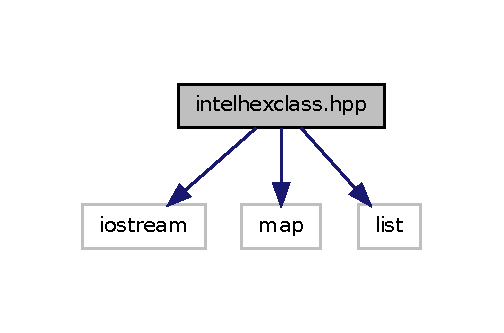
\includegraphics[width=242pt]{intelhexclass_8hpp__incl}
\end{center}
\end{figure}
This graph shows which files directly or indirectly include this file:\nopagebreak
\begin{figure}[H]
\begin{center}
\leavevmode
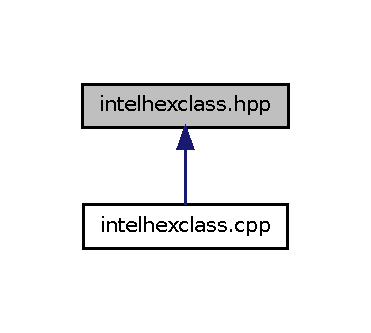
\includegraphics[width=178pt]{intelhexclass_8hpp__dep__incl}
\end{center}
\end{figure}
\subsection*{Classes}
\begin{DoxyCompactItemize}
\item 
class \hyperlink{classintelhex}{intelhex}
\begin{DoxyCompactList}\small\item\em Class to decode, encode and manipulate Intel HEX format files. \item\end{DoxyCompactList}\end{DoxyCompactItemize}


\subsection{Detailed Description}
\begin{DoxyAuthor}{Author}
Stuart Cording aka CODINGHEAD
\end{DoxyAuthor}
A class to handle the encoding, decoding and manipulatio of an Intel HEX format file as generated by many tool chains for embedded processors and microcontrollers.

This class is constructed based upon the definition given in the document 'Hexadecimal Object File Format Specification', Revision A, January 6, 1988, © 1998 Intel Corporation.

\begin{DoxyNote}{Note}
See the git versioning notes for version information 
\end{DoxyNote}


Definition in file \hyperlink{intelhexclass_8hpp_source}{intelhexclass.hpp}.


\printindex
\end{document}
